\documentclass[11pt]{article}
\usepackage{times}

\usepackage{fullpage}

\usepackage{ifpdf}

\ifpdf
\usepackage[pdftex]{graphicx}
\else
\usepackage{graphicx}
\fi

\ifpdf
\DeclareGraphicsExtensions{.pdf,.jpg,.tif}
\else
\DeclareGraphicsExtensions{.eps,.jpg}
\fi

\newcommand{\lare}{{\it LareXd}\ }
\newcommand{\visit}{VisIt\ }

\begin{document}
\title{
\bfseries\scshape LareXd User Guide}
\author{\bfseries\itshape Tony Arber\thanks{E-mail address: T.D.Arber@warwick.ac.uk}\\
University of Warwick, Department of Physics, Coventry, CV4 7AL, UK}
\date{Version 2.11}
\maketitle

\thispagestyle{empty}

\section*{Abstract}
{\it LareXd} are Lagrangian remap codes for solving the MHD equations in 2 or 3D. The code uses a staggered grid and is second order accurate in space and time. The use of shock viscosity and gradient limiters make the code ideally suited to shock calculations. This document describes how to obtain, make and run the {\it LareXd}  codes. The instructions are aimed at code users, not developers, although some references to more detailed numerics are included.


%---------------------------------------------------------------------------------------------------------------
\section{Introduction}
The Lagrangian remap code comes in 2D ({\it Lare2d}) and 3D ({\it Lare3d}). For convenience when referring to either code this is called the {\it LareXd} code. A detailed description of the algorithm has been published \cite{jcp} along with test cases. Note however that the latest version of the code uses a different form of shock viscosity and resistivity to that documented in JCP. The latest version of the code, and of this manual, can be obtained from CCPForge {\tt http://ccpforge.cse.rl.ac.uk/}.

Without going into detail, see \cite{jcp} for complete algorithm, the main features of the code are:
\begin{itemize}
 \item Solves the nonlinear MHD equations with user controlled viscosity and resistivity. Optional physics packages are: gravity, the Hall term (only in 2D), partially ionised hydrogen equation of state, Cowling resistivity, parallel thermal conductivity optimically thin radiative losses and user specified heating functions.
 \item Splits each timestep into a Lagragrian step followed by a remap onto the original grid. This allows all of the physics to be included into a simple Lagrangian step making it easy to add additional physics. The remap step includes gradient limiters to ensure the correct shock solution.
 \item Uses a staggered grid to prevent the checkerboard instability and to build conservation laws into the finite difference scheme, i.e. it is a compatible difference scheme in Lagrangian numerical jargon.
 \item Parallelised via MPI and known to scale linearly.
 \item Comes with packages for visualisation by IDL and VisIt. \cite{visit}
\end{itemize}

This manual should be sufficient to set up {\it LareXd} for any initial conditions, run the code and begin analysing the results. In order to do this you must know the core equations that are solved. It is also essential that you know something about the code structure and once the code has run how to load the data into IDL or VisIt. For the more ambitious you will need a good understanding of the Lagrangian step as this is what you will need to change to include additional physics. It is unlikely you will ever need to know how to change the remap step. If editing the core code note that this is always in normalised form so you must understand how this is applied. For examples of the uses of the {\it LareXd} codes just check out papers that reference \cite{jcp}. In order that this manual does not get stuck in the fine details of shock theory etc. it has been written in an informal style which deliberately oversimplifies some theoretical points. It's a user manual, not a theoretical treatise. References to grown up theory are at the end.



\section{Equations and Normalisation}

{\it LareXd} includes options to run with partially ionised hydrogen and the Hall term (only in 2D). Other options are being added. In order to get used to using the code, and to make the initial description easier, these options are moved to the next section. Here we concentrate just on standard resistive MHD. In almost all cases the code should be run with viscosity, either real or shock viscosity, but how this is treated is postponed until later to keep the first steps easier. In S.I. units the standard resistive MHD equations are

\begin{eqnarray}
\frac{\partial \rho}{\partial t}&=&- \nabla\cdot(\rho \mathbf{v})\\
\frac{\mathrm{D}\mathbf{v}}{\mathrm{D}t}&=&\frac{1}{\rho}\mathbf{j}\times\mathbf{B}
-\frac{1}{\rho}\nabla P\\
\frac{\partial \mathbf{B}}{\partial t}&=&-\nabla\times\mathbf{E} \label{faraday}\\
\frac{\mathrm{D}\epsilon}{\mathrm{D}t}&=&-\frac{P}{\rho}\nabla\cdot\mathbf{v}+\frac
{\eta}{\rho}j^{2}\\
\mathbf{E}+\mathbf{v}\times\mathbf{B}&=&\eta \mathbf{j} \label{ohm}\\
\nabla\times\mathbf{B}&=&\mu_0 \mathbf{j}
\end{eqnarray}

Where $\mathrm{D}/\mathrm{D}t$ is the advective derivative and all other terms have their usual meaning. Ideal MHD is recovered simply by setting $\eta$, the resistivity, to zero. Note in these equations $\eta$ is resistivity, not magnetic diffusivity, so that $\eta=1/\sigma$ where $\sigma$ is the conductivity. Note that the energy equation is written in terms of the specific internal energy density $\epsilon$. There are good numerical reasons for doing this which go beyond the scope of this introduction. Definitions you may find useful for converting between $\epsilon$ and the more familiar pressure and temperature are
\begin{eqnarray*}
P&=&\frac{\rho k_{B}T}{\mu_m}\\
\epsilon&=&\frac{P}{\rho(\gamma-1)}=\frac{k_B T}{\mu_m (\gamma-1)}
\end{eqnarray*}
where $\mu_m$ is the reduced mass, i.e. the average mass of all particles in the plasma. Hence $\mu_m=m_p$ for neutral hydrogen atoms ($m_p$ is the proton mass) and $\mu_m=0.5 m_p$ for fully ionised hydrogen.

There are two occasions when you will need to understand the normalisation. The first is to input your variables in dimensionless form. To do this of course you must have chosen a normalisation. For some additional physics packages to work correctly you must tell {\it LareXd} the numerical values of your normalising length, magnetic field and mass density (more on this below). The additional physics packages that require this are thermal conduction, optically thin radiative losses and the inclusion of neutrals. If you are only running resistive MHD then these are not needed. The second reason you may need to understand the normalisation is that all of the core code works on the normalised equations so that should you want to edit the code, e.g. to change the resistivity, you must do this on normalised equations.

The normalisation is through the choice of normalising magnetic field $B_0$, density $\rho_0$ and length $L_0$. Thus we define dimensionless quantities as
\begin{eqnarray*}
x&=&L_0 \hat{x}\\
\mathbf{B}&=&B_0\hat{\mathbf{B}} \\
\rho&=&\rho_0 \hat{\rho}
\end{eqnarray*}
These three basic normalising constants are then used to define the normalisation for velocity, pressure, time, current density, electric field, temperature, reduced mass and specific internal energy density through
\begin{eqnarray*}
v_{0}&=&\frac{B_{0}}{\sqrt{\mu_{0}\rho_{0}}}\\
P_{0}&=&\frac{B^{2}_{0}}{\mu_{0}} \\
t_0&=&\frac{L_0}{v_0}\\
j_{0}&=&\frac{B_{0}}{\mu_{0}L_{0}}\\
E_0&=&v_0 B_0\\
T_0&=&\frac{\epsilon_0 \bar{m}}{k_B}\\
\mu_{m0}&=&\bar{m}\\
\epsilon_0&=&v_0^2
\end{eqnarray*}
so that $\mathbf{v}=v_0\hat{\mathbf{v}}$, $\mathbf{j}=j_0\hat{\mathbf{j}}$, $t=t_0\hat{t}$ and $P=P_0\hat{P}$ etc. In these equations $\bar{m}$ is the average mass of ions in the plasma, i.e. $\bar{m}=m_p$ for pure hydrogen but  $\bar{m}=1.2 m_p$ is typical for the Solar corona. Thus $\bar{m}$ is actually an input parameter to the code and is set in the \texttt{control.f90} file (see later). Applying this normalisation to the ideal MHD equations simply removes the vacuum permeability $\mu_0$. Note if you would like to fix a normalising temperature this means that you must choose $L_0,\rho_0, B_0$ so that the calculated $T_0$ gives the required temperature normalisation.

For resistive MHD substitute equation \ref{ohm} into \ref{faraday} and apply the normalisation to get
\begin{displaymath}
 \frac{\partial \hat{\mathbf{B}}}{\partial \hat{t}}=\hat{\nabla}\times(\hat{\mathbf{v}}\times\hat{\mathbf{B}})
	-\frac{1}{\mu_0 L_0 v_0}\hat{\nabla}\times(\eta\hat{\nabla}\times\hat{\mathbf{B}})
\end{displaymath}
Note that the resistivity is not assumed spatially uniform in {\it LareXd}. This leads naturally to the normalisation of resistivity of
\begin{displaymath}
 \hat{\eta}=\frac{\eta}{\mu_0 L_0 v_0}
\end{displaymath}
or $\eta_0=\mu_0 L_0 v_0$. Since $v_0$ is the normalised Alfv\'en speed this means that $\hat{\eta}=1/S$ where $S$ is the Lundquist number. This resistivity can either be uniformly applied or triggered when the current density exceeds a threshold value. This can be controlled in the \texttt{control.f90} file.

Dropping all of the hats on normalised variables the final normalised resistive MHD equations, in Lagrangian form, are
\begin{eqnarray}
\frac{\mathrm{D}\rho}{\mathrm{D}t}&=&-\rho \nabla\cdot \mathbf{v}\\
\frac{\mathrm{D}\mathbf{v}}{Dt}&=&\frac{1}{\rho}(\nabla\times\mathbf{B})\times\mathbf{B}
-\frac{1}{\rho}\nabla P \label{velocity_eqn}\\
\frac{\mathrm{D}\mathbf{B}}{\mathrm{D}t}&=&(\mathbf{B}\cdot\nabla)\mathbf{v}-\mathbf{B}
(\nabla\cdot\mathbf{v})-\nabla\times(\eta\nabla\times\mathbf{B})\\
\frac{\mathrm{D}\epsilon}{\mathrm{D}t}&=&-\frac{P}{\rho}\nabla\cdot\mathbf{v}+\frac
{\eta}{\rho}j^{2} \label{energy_eqn}
\end{eqnarray}

Where $\epsilon$ is the specific internal energy density, $P = \rho \epsilon(\gamma - 1)$ and $\gamma$ is the ratio of specific heats - again this is specified in \texttt{control.f90}.

The fact that the thermal pressure is normalised to the reference magnetic pressure means that there is no plasma $\beta$ in the code. It does not mean that the code must have a magnetic field. $B_0$ is the normalising field. It is then perfectly acceptible to set $\mathbf{B}=0$ as this is really fixing $\hat{\mathbf{B}}$ and has no effect on  $B_0$. The temperature is not needed to solve the resistive MHD equations and as a result no explicit temperature normalisation is needed to solve the resistive MHD equations. However it is often convenient to specify initial conditions in terms of temperature and this must be converted to specific internal energy density before the first timestep.

{\it LareXd} is set up with gravity assumed downwards in the $z$ direction. It's trivial to change the direction in the \texttt{lagran.f90} file. In normalised units the momentum equation for the $z$ component is therefore given by
\begin{displaymath}
 \frac{\mathrm{D}\mathbf{v}}{Dt}=\frac{1}{\rho}(\nabla\times\mathbf{B})\times\mathbf{B}
-\frac{1}{\rho}\nabla P-\hat{g}
\end{displaymath}
where $\hat{g}=L_0 g / v_0^2$. In {\it LareXd} $\hat{g}$ is only a function of $z$, i.e. it is a 1D array, and it does not change in time. Note also that gravity is defined on the cell vertex, i.e. the same location as all components of velocity. More on this later when the computational grid is defined.

\subsection{Viscosity}
Viscosity is added through the stress tensor $\sigma_{ij}$ and strain rate $\varepsilon_{ij}$ which add an additional force onto the $i$ component of the momentum equation
\begin{displaymath}
\frac{\mathrm{D}v_i}{Dt}=\frac{1}{\rho}\frac{\partial \sigma_{ij}}{\partial x_j}
\end{displaymath}
and an associated heating term
\begin{displaymath}
\frac{\mathrm{D}\epsilon}{Dt}=\frac{1}{\rho}\varepsilon_{ij}\sigma_{ij}
\end{displaymath}
In order to ensure that the stress tensor is zero under uniform rotation or compression it must be isotropic and traceless
\begin{eqnarray*}
\sigma_{ij} &=& 2 \nu \left(\varepsilon_{ij}-\frac{1}{3}\delta_{ij}\nabla\cdot\mathbf{v}\right) \\
\varepsilon_{ij} &=& \frac{1}{2}\left(\frac{\partial v_i}{\partial x_j} + \frac{\partial v_j}{\partial x_i} \right)
\end{eqnarray*}
As with the normalisation of the resistivity when the normalisation procedure above is applied the viscosity $\nu$ above is replaced by $\hat{\nu}$ such that
\begin{displaymath}
 \hat{\nu}=\frac{\nu}{\rho_0 L_0 v_0}
\end{displaymath}
Since $v_0$ is the normalised Alfv\'en speed this means that $\hat{\nu}=1/R$ where $R$ is the Reynolds number defined using the Alfv\'en speed. Note that in {\it LareXd}  $\hat{\nu}$ is called {\it visc3}. In practice $\nu$ is often limited by the numerical resolution but should you wish to calculate a real $\nu$ for a real physical problem remember not to confuse viscosity and kinematic viscosity. The kinematic viscosity is defined as $\nu/\rho$.

For fully ionised plasma with no magnetic field the bulk plasma viscosity is proportional to $\rho T \tau_i$ \cite{nrl} where $\tau_i$ is the ion collision time. Since $\tau_i \propto T^{3/2}/\rho$ this means the real viscosity, in the absence of a magnetic field, should vary as
\begin{displaymath}
  \nu \propto T^{5/2}
\end{displaymath}
and therefore does not depend on density. However the majority of people working in MHD for space and astrophysics never want to use the real viscosity but instead have an equation of the form $\partial_t v = - \nu \nabla^2 v$, suitable for incompressible flows, with constant $\nu$. So that the viscosity in {\it Lare} reduces to this form the viscosity internally is defined to be proportional to density. Since this is divided by density in the momentum equation this will reduce to the simple incompressible form if the density is uniform. Should you wish to use real viscosity then you must make {\it visc3} a function of space and include the correct density and temperature dependence. To do this note that the stress tensor is labelled as, for example, \texttt{qxy} with the \texttt{q} read as $\sigma$ so that $\sigma_{x,y}$ in the code is \texttt{qxy}. These are defined inside \texttt{SUBROUTINE viscosity\_and\_b\_update} in \texttt{lagran.F90}.


\subsection{Shock viscosity}
At shocks the gradients become singular and the differential equations are not defined. Instead we can use the integrated form of the equations to get jump conditions across shocks. To keep things simple let's just consider the 1D Euler equations, i.e. ideal MHD with $\mathbf{B}=0$. The jump condition for the pressure across the shock is
\begin{equation}
P_1-P_0=\frac{\gamma+1}{4}\rho_0(\Delta v)^2 + \rho_0 |\Delta v|\left[\left(\frac{\gamma+1}{4}\right)^2(\Delta v)^2 + c_s^2\right]^{1/2}\label{jump}
\end{equation}
where $P_1$ is the pressure behind the shock, $P_0$ is the pressure in front of the shock, $c_s$ is the sound speed and $\Delta v$ is the jump in velocity across the shock. Any finite differencing of the fluid equations higher than first order accurate will introduce false oscillations behind the shock unless something is done to reconcile those difference equations with the jump condition above. The jump in entropy associated with the shock is not zero, however the Euler equations are ideal and contain no dissipation. To introduce some dissipation, but only at steep gradients, consistent with the jump conditions we can add a scalar $q$ to $P$ when computational cells are compressed. Noting that in 1D $\Delta v=\Delta x \nabla\cdot\mathbf{v}$, where $\Delta x$ is the cell size, we add to each cell
\begin{displaymath}
q = \nu_1 \rho c_s \Delta x |\nabla\cdot\mathbf{v}| + \nu_2 \rho \Delta x^2 (\nabla\cdot\mathbf{v})^2
\end{displaymath}
provided that $\nabla\cdot\mathbf{v}<0$, i.e. the cell is being compressed. Since this is added to the pressure there is an associated heating term added to equation \ref{energy_eqn} of $-q \nabla\cdot\mathbf{v}/\rho$. Note that $q$ is always positive and hence we must insist it is only applied when $\nabla\cdot\mathbf{v}<0$ to ensure that shocks only ever heat. The coefficients $\nu_1$ and $\nu_2$ are fixed by experimenting but usually $\nu_1=0.1$ and $\nu_2=0.5$ does a good job. By construction $\nu_1$ and $\nu_2$ are dimensionless. In smooth regions of the solution in the limit of increasing resolution $\nabla\cdot\mathbf{v}$ is finite and $\Delta x$ tends to zero so that $q$ vanishes. However at shocks $\Delta x \nabla\cdot\mathbf{v}=\Delta v$, the velocity jump across the shock, and $q$ remains finite. Therefore as the resolution is increased $q$ is only applied at shocks, it is only ever heating and has the functional form required to slightly diffuse the shock and reproduce the jump condition for pressure. If you've got to this point and think this is all a bit hand waving then good. If you want to study the grown up derivation then hit the library and references at the end of this manual.

The above principle generalises easily to 3D Euler simulations except that now the scalar which is added to the pressure in each cell is
\begin{equation}
q = \nu_1 \rho c_s L|s| + \nu_2 \rho L^2 s^2 \label{qmono}
\end{equation}
$s$ is the rate of strain tensor in the direction normal to the shock front \cite{wilkins}. Again this is only applied to cell with $\nabla\cdot\mathbf{v}<0$ so that $-q \nabla\cdot\mathbf{v}$ heating is positive. The only change is that the scale length used is no longer just $\Delta x$. The $L$ in this formula is the distance across the cell in the direction normal to the shock front. This prevents the shock viscosity from introducing grid scale noise and preserves circular shocks on the Cartesian grid. The full theory for this can be found in \cite{wilkins}. When $L$ is used the shock viscosity is still just a scalar even though we are working in 2 or 3 dimensions. This technique is often called Wilkins $q_{mono}$ viscosity which may help to explain some of the compiler directive names. $q_{mono}$ viscosity is the minimum requirement for fluid shock viscosity and is often all that is needed.

The above is fine for non-MHD problems. If the derivation of the shock jump conditions is repeated for MHD then no simple version of equation \ref{jump} drops out. In simplified cases, e.g. 1D problems with the magnetic field in the ignoreable direction, similar expressions to equation \ref{jump} can be derived and these have lead to some people using  equation \ref{qmono} but with $c_s$ replaced by the fast magnetoacoustic speed $c_f$. This is what you get in {\it LareXd} if you use the \texttt{QMONO} precompiler option. However, since this is a scalar which is added to the pressure it has no control over the shear forces which can come into play in MHD shocks. To deal with such possibilities the {\it LareXd} codes, by default, use a tensor shock viscosity. This is a hybrid between the $q_{mono}$ and the real tensor viscosity described above. The only  justification is that it has the correct tensor properties and is only applied at shocks. This tensor shock viscosity is

\begin{equation}
\sigma_{ij}^{shock} =  (\nu_1 \rho c_f L + \nu_2 \rho L^2 |s|)  \left(\varepsilon_{ij}-\frac{1}{3}\delta_{ij}\nabla\cdot\mathbf{v}\right)   \label{shock}
\end{equation}
This is applied to all cells, not just those which are compressed, as significant shear forces may exist across expanding cells. The heating term is however always positive.

{\bf N.B.} The tensor viscosity, both shock and real, are known to fail with extreme grid aspect ratios, i.e. cells which are far from being square. The precise value of cell aspect ratio which is acceptable is problem dependent. High aspect ratio cells should be avoid for accuracy reasons anyway but if you do have highly elongated cells and notice problems with the code mysteriously hanging at some point try either no viscosity or $q_{mono}$. You will have to experiment to work out when or if this is needed.

\subsection{Boundary Conditions}
Boundary conditions can be set in {\tt control.f90}. The preset routines are periodic, open and other. If you specify {\tt other} then you must be sure that what is in {\tt boundary.f90} matches precisely your imposed conditions - take care in getting the grid staggering right. Open boundary works on a simplified far-field characteristic model. For this it is best to test on your problem, if fine then go ahead and use. However if these do not work for you problem, they are not guaranteed to work well for all conditions, then you may have to resort to coding up your own conditions in {\tt boundary.f90} and using {\tt other} as your choice for boundaries.

All choices of boundary also allow damping to be applied near the boundary. This is entirely user configurable and requires that the appropriate boundaries are treated as you prefer in {\tt damp\_boundaries} inside {\tt boundary.f90}.

\section{Hall MHD}
The 2D version {\it Lare2d} comes with an input deck option to run using Hall MHD. In Hall MHD the only difference in the basic equations is that Ohm's law changes from
\begin{displaymath}
\mathbf{E}+\mathbf{v}\times\mathbf{B}=\eta \mathbf{j}
\end{displaymath}
to
\begin{displaymath}
\mathbf{E}+\mathbf{v}\times\mathbf{B}-\frac{1}{n_e e}\mathbf{j}\times\mathbf{B}=\eta \mathbf{j}
\end{displaymath}
where $n_e$ is the electron number density. This can also be written as
\begin{displaymath}
\mathbf{E}+\mathbf{v_e}\times\mathbf{B}=\eta \mathbf{j}
\end{displaymath}
where $v_e$ is the electron fluid velocity. This seemingly minor change has a dramatic effect on running {\it Lare2d} due to the dispersion relation for Whistler waves. As a result experience has shown that it is usually best to not have a stretched grid for these simulations and keep the computational cells as square as possible. An example of the application of Hall MHD can be found in \cite{hall}. Introducing the Hall term also brings in another dimensionless parameter. This can be seen from making the Hall Ohm's law dimensionless
\begin{displaymath}
\hat{\mathbf{E}}+\hat{\mathbf{v}}\times\hat{\mathbf{B}}-\frac{m_iB_0}{\mu_0 L_0 e v_0 \rho_0} \frac{\hat{\mathbf{j}}\times\hat{\mathbf{B}}}{\hat{\rho}}=\hat{\eta} \hat{\mathbf{j}}
\end{displaymath}
The new parameter in front of the Hall term is the ratio of the characteristic ion inertial depth $\lambda_i$ to the normalising scalelength $L_0$. The ion inertial depth can be written in a number of ways, e.g.
\begin{displaymath}
\lambda_i=\frac{m_i B_0}{\mu_0 e v_0 \rho_0} =\left(\frac{m_i^2}{\rho_0\mu_0e^2}\right)^{1/2}=\frac{m_i v_0}{e B_0}=\frac{c}{\omega_{pi} }
\end{displaymath}
where $c$ is the speed of light and
\begin{displaymath}
\omega_{pi}=\left(\frac{n_0 e^2}{m_i \epsilon_0}\right)^{1/2}
\end{displaymath}
is the ion plasma frequency. Once the density is normalised, through the mass density, $n_0$ is known and thus $\lambda_i$ is not a free parameter. It is however treated as a free parameter in \texttt{control.f90} as it is often interesting to inflate $\lambda_i$, much as one does for the resistivity, for computational reasons. As a result care must be taken when choosing $\lambda_i$. In the code you must specify {\tt lambda\_i} which is $\lambda_i/L$.

If Hall MHD is turned on in \texttt{control.f90} then {\tt lambda\_i} must be specified inside the initial conditions. Note that like gravity {\tt lambda\_i} is a function of space. This is important as there are occasions, such as reflecting wall boundary conditions, when you must set {\tt lambda\_i} on the boundary. Note also that {\tt lambda\_i} is defined at cell vertices and you need to specify all values in the range {\tt lambda\_i(0:nx, 0:ny)}.

\section{Partial Ionisation and Cowling Resistivity}
{\it Lare3d} has an option to include partial ionisation. The equations this solves are documented in \cite{flux-emergence}. All of this physics is included in the file \texttt{neutral.f90}. Key to these routines is the calculation of the neutral fraction $\xi_n$ which is the ratio of the mass density of the neutral gas to the total mass density. For now let's assume that $\xi_n$ is known. $\xi_n$ affects the basic equations in a number of ways. At the simplest level it changes the partial pressures so that now the equation of state is different to that of ideal MHD. There are three options for the equations of state determined by setting \texttt{eos\_number} in \texttt{control.f90}
\begin{itemize}
\item \texttt{eos\_number=EOS\_IDEAL}: These have been explained above and are repeated here for easy comparison
\begin{eqnarray*}
P&=&\frac{\rho k_{B}T}{\mu_m}\\
\epsilon&=&\frac{P}{\rho(\gamma-1)}\\
\mu_m&=&\bar{m}\ m_{reduced}
\end{eqnarray*}
The reduced mass is controlled through the logical variable {\tt neutral\_gas} in  \texttt{control.f90}. If
{\tt neutral\_gas = .TRUE.} then $m_{reduced}=1$, if {\tt neutral\_gas = .FALSE.} then $m_{reduced}=0.5$.
Thus setting $m_{reduced}=1$ gives un-ionised atomic hydrogen while $m_{reduced}=0.5$ will give fully ionised hydrogen.

\item \texttt{eos\_number=EOS\_PI}: Here the effect of neutrals on the partial pressures is included
\begin{eqnarray*}
P&=&\frac{\rho k_{B}T}{\mu_m}\\
\epsilon&=&\frac{P}{\rho(\gamma-1)}\\
\mu_m&=&\frac{\bar{m}}{2-\xi_n}
\end{eqnarray*}

\item \texttt{eos\_number=EOS\_ION}: This includes the full partial pressures and the ionisation energy.
\begin{eqnarray*}
P&=&\frac{\rho k_{B}T}{\mu_m}\\
\epsilon&=&\frac{P}{\rho(\gamma-1)}+(1-\xi_n)\frac{X_i}{\bar{m}}\\
\mu_m&=&\frac{\bar{m}}{2-\xi_n}
\end{eqnarray*}
where $X_i$ is the ionisation energy for hydrogen.

\end{itemize}

Note that we always assume an ideal gas so the first equation is the same for all options. For an ideal plasma we assume a single ionisation state so that the reduced mass is half the ion mass. If including the effect of neutrals fully one should always use \texttt{eos\_number=EOS\_ION} as the ionisation energy of hydrogen must be taken into account. The second option is therefore never formally correct. It is however retained as the energy equation used in MHD is often missing important sources and sinks and therefore having the option to include this term is sometimes useful for sensitivity studies. This is explained in \cite{flux-emergence}.

All of the above assumes that $\xi_n$ is known. This is specified in \texttt{neutral.f90}. In this version of the code $\xi_n$ is determined from a modified Saha equation based on a three level hydrogen model \cite{brown}. This is therefore only even approximately valid for an averaged quiet solar chromosphere. To change this the routines that need to return, or calculate, a different $\xi_n$ are \texttt{get\_neutral} and \texttt{neutral\_fraction} in \texttt{neutral.f90}. The current code assumes that below a height of zero is the sub-photospheric plasma. This is in LTE and thus the dilution factor and local ration temperature are changed in \texttt{get\_neutral} if this is true.

As well as affecting the partial pressure the neutral fraction can alter the nature of resistive effects. The dominant term here is the introduction of an anisotropic resistivity so that the Ohm's law becomes
$\mathbf{E}+\mathbf{v}\times\mathbf{B}=\eta \mathbf{j_{\parallel}} + \eta_c \mathbf{j_{\perp}}$
where $\eta_c$ is the Cowling resistivity which may be orders of magnitude larger than the Spitzer value. Once $\xi_n$ is known $\eta_c$ can be calculated from the standard formula in \cite{flux-emergence}. This is done in subroutine \texttt{perpendicular\_resistivity} in \texttt{neutral.f90}.

\section{Thermal Conduction} % (fold)
\label{sec:thermal_conduction}
Thermal conduction in LARE is based on the Braginskii thermal conduction in the presence of a magnetic field and is of the form\\
\[
\frac{\partial \epsilon}{\partial t} = \nabla . \left(\left(\kappa \frac{\vec{B}}{B^2+b_{min}^2}. \nabla T\right) \vec{B} \right) +  \nabla . \left(\kappa  \frac{b_{min}^2}{B^2+b_{min}^2}  \nabla T \right)
\]
where $\kappa = \kappa_0  T^\frac{5}{2}$. In the limit $b_{min}\to 0$ this recovers the Braginskii parallel thermal conductivity. Finite $b_{min}$ is used to make the conductivity isotropic when $B=0$.  How this is implemented is described in the Appendix. Note that $\kappa_0$ is hard coded to $10^{-11}$ and therefore this routine only works if you have set {\tt B0, L0, RHO0} in {\tt control.f90} correctly. If you want to just pick the thermal conductivity, i.e. make it up and generate unphysical results, then you can do this by changing $\kappa_0$ which is set in {\tt SUBROUTINE set\_normalisation} in {\tt src/core/normalise.f90}.

Depending on your problem you may need to change $b_{min}$ which is set as a constant (parameter) in {\tt src/core/conduct.f90}. It is also possible to control the fractional accuracy of the SOR Gauss-Seidel scheme that is used to update the temperature, this is also in {\tt src/core/conduct.f90} and a value of $10^{-5}$ is known to reproduce analytic results well. If runtime becomes an issue this can be reduced but then you will need to test more carefully.

% section thermal_conduction (end)

\section{Open  Boundaries} % (fold)
\label{sec:open_bcs}
Open boundaries are now implemented via far-field Riemann characteristics. This calculates the slow, fast, Alfven etc. speeds and then projects 1D Riemann invariants into ghost cells. If the wave is outgoing values are propagated from the inside the domain into the ghost cells. If the waves are inward propagating then values are carried in from the far-field. This requires a fixed far-field, i.e. specified values of $\rho, \epsilon, v_x, v_y, B_x, B_y, B_z$. So that the open boundary conditions doesn't affect the initial equilibrium these are set to the ghost cell values as defined in the initial conditions. As a result these open boundaries are only accurate if the magnetic field does not change a lot from the initial field. More accurately the far-field specified at $t=0$ must be a valid far-field later in the simulation. Otherwise the far-field problem for MHD is not well posed.

{\it Notes:} In this version these routines have been tested with simple straight fields and x-point fields and they seem robust. Reflection is typically a few percent but can be as large as 10\% in extreme cases. It is best to just try for your problem and see if they work. If not let me know so I can either look to fix the problem or list the initial conditions here as one's which are known not to work. If the open boundaries do fail then the best option is to use a stretched grid with a damping layer. Sometimes simply commenting out the line {\tt CALL open\_bcs} can help! Most of these problems are to do with the open boundary problem for MHD not being well posed so in all these cases you will be conditioning the solution so caution is needed.

The open boundaries have not been tested with resistivity or thermal conductivity. If this causes problems be sure that resistivity is zero at the boundary. Also the open boundaries do not work with gravity. Open boundaries with gravity should be OK on surfaces of constant potential gravitational potential but not always otherwise. At the lower boundary care must be taken to not let the solution fall through the bottom. Experiment to find the best approach. If all fails use damping regions or contact me directly.

% section open_bcs (end)





\section{The Grid}
In order to define the initial conditions and understand the location of output arrays in physical space it is vital that all users know the underlying structure of the grid. This is best explained by stepping up through 1D then 2D and finally 3D computational cells. In 1D there are $nx$ computational cells. These are labelled from $ix=1$ up to $ix=nx$. The variables used in the code are not defined at the same point in a cell. We therefore need to be able to access the location of different parts of the grid to set up the initial conditions. For this $xb_i$ is the position of the right hand boundary of a cell and $xc_i$ the position of the cell centre. This means that the left hand boundary of the computational domain is at $xb_0$. The width of each cell is $dxb_i$ and the distance between cell centres is $dxc_i$. In this coordinate system the velocities are all defined at the cell boundaries and all scalars (density, pressure, specific internal energy density) are defined at cell centres. This is shown in figure \ref{1d-staggered}. The magnetic field components are defined at different locations for each component. $B_x$ is defined at the cell boundary ($xb_i$) while the $B_y$ and $B_z$ components are cell centred. Note that this staggering is essential for the accuracy, and conservation properties, of {\it LareXd}.

One side effect of this staggering that can cause confusion is that to define the initial conditions inside the computational domain more points are needed for velocities and $B_x$ than for the scalars and other magnetic field components. This is because you must define, for example, $v_x$ from $ix=0$ to $ix=nx$ but only need the density from $ix=1$ to $ix=nx$. Note that the grid spacing need not be uniform so that $dxb_i$ need not equal $dxb_{i+1}$. The default setup of the grid is uniform but if the flag \texttt{x\_stretch=.TRUE.} is set in \texttt{control.f90} then the grid will be non-uniform.


\begin{figure}
\begin{center}
  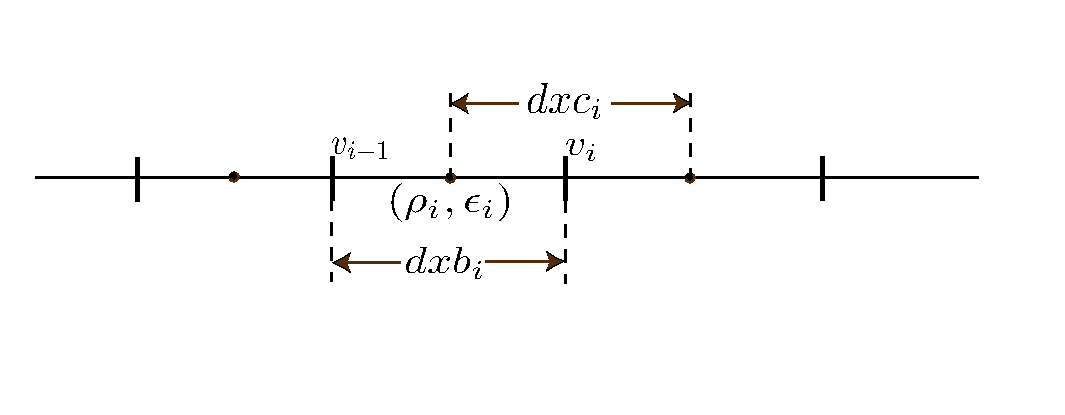
\includegraphics{1d-staggered-grid.pdf}
\caption{1D Staggered Grid}
\end{center}
\label{1d-staggered}
\end{figure}

In 2D the velocities are defined at cell corners, the scalars and ignorable direction magnetic field at cell centres. The remaining magnetic field components are defined at cell edges. This is shown in figure \ref{2d-staggered}. When analysing output it is OK to define the kinetic energy density as $0.5\rho_{ij}v_{ij}^2$ but the accurate estimate of kinetic energy should make sure that these variables are defined at the same place. In figure \ref{2d-staggered} the mass density at the vertex ($\rho_{ij}^v$) is also shown and once defined the kinetic energy density is then  $0.5\rho_{ij}^v v_{ij}^2$. To get the vertex density you must average the densities in the four surrounding cells. Since the grid is possibly stretched care should be taken with these averages and it is best to define the vertex density by summing up the total mass in the surrounding four cells and dividing by the total area. This sort of thing is done a lot inside the code but in most cases this isn't important to users of the code. It is flagged here just as a warning for calculating products of output variables which are not defined at the same location. The Hall term is especially sensitive to this and great care should be taken calculating derived quantities on the staggered grid if doing Hall MHD work.

\begin{figure}
\begin{center}{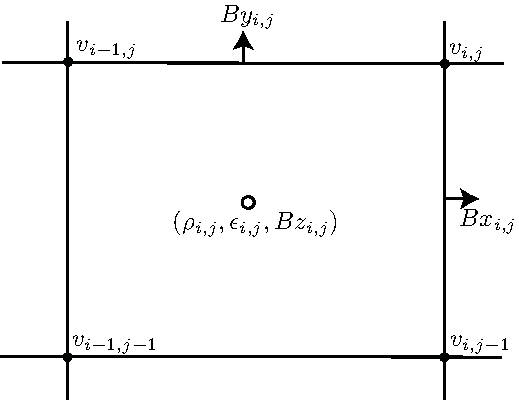
\includegraphics{2d-staggered-grid.pdf}}\end{center}
\caption{2D Staggered Grid}
\label{2d-staggered}
\end{figure}

Once you have grasped the 2D grid then 3D is obvious. This is shown in figure \ref{3d-staggered}. Here scalars are volume centred, velocities are defined at cell vertices and magnetic field components are defined as face centred. Gravity is a function only of the $z$ coordinate and is define at the cell vertices, i.e. same location as the velocity.
\begin{figure}
\begin{center}{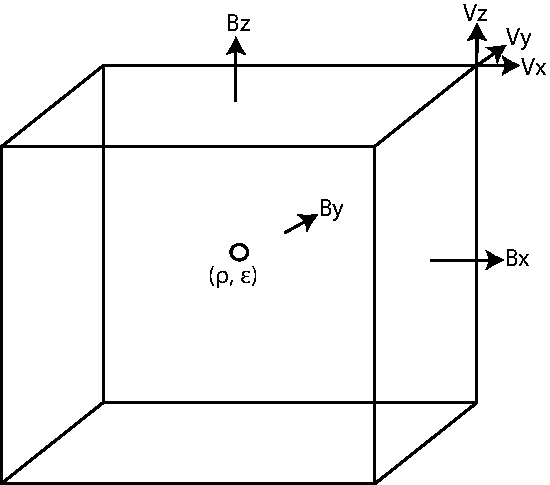
\includegraphics{3d-staggered-grid.pdf}}\end{center}
\caption{3D Staggered Grid}
\label{3d-staggered}
\end{figure}

\subsection{Stretched Grids}
You can choose to stretch the grid. If you do this the grid can be stretched differently in each of the three directions. The routines for defining the stretched grids are in \texttt{setup.F90} and are imaginatively called \texttt{stretch\_x}, \texttt{stretch\_y}, and \texttt{stretch\_z}. Taking \texttt{stretch\_x} as an example, when this is called the boundaries of the cells
$xb_i$ are defined as uniformly spaced from \texttt{x\_min} to \texttt{x\_max} as defined in \texttt{control.f90}. For reasons to do with the MPI parallelism these are called \texttt{xb\_global} at this point. The subroutine \texttt{stretch\_x} is free to redistribute these boundaries however you like but note that if the routine changes the overall size of the domain then you should reset the variable \texttt{length\_x}. Here's an example of a stretching function
\begin{verbatim}
   SUBROUTINE stretch_x
   ! replace with any stretching algorithm as needed
    REAL(num) :: width, dx, L, f, lx_new
    lx_new = 200.0_num
    ! new total length
    L = length_x / 2.0_num
    ! centre of tanh stretching in unstretched coordinates
    width = length_x / 10.0_num
    ! width of tanh stretching in unstretched coordinates
    f = (lx_new - length_x)/(length_x - L)/2.0_num
    dx = length_x / REAL(nx_global,num)
    dxnew = dx+f*(1.0_num+TANH((ABS(xb_global)-L)/width))*dx
    DO ix = 1, nx_global+2
       xb_global(ix) = xb_global(ix-1) + dxnew(ix)
    ENDDO
    length_x = xb_global(nx) - xb_global(0)
  END SUBROUTINE stretch_x
\end{verbatim}
Don't ask me why this function is written this way, I can't remember. All that you need to know is what you want to do and then you're on your own. Good luck! One word of advice: if you stretch the grid so that the cells are far from square or the $dxb_i$'s change by more than 10\% from cell to cell then you cannot expect an accurate solution in that region of the computational domain. Do not use a stretched grid with the Hall term as the dispersion relation for Whistler waves means it is very likely that grid scale noise will develop and reflect back off the stretching. As a rule only stretch the grid if you absolutely must and don't overdo the stretching.

\section{Code Structure}
The code is all stored in the \texttt{src} sub-directory. This contains two sub-directories \texttt{core, Old}. The files have either a \texttt{.f90} or \texttt{.F90} extension. The ones with \texttt{.F90} are those which contain pre-compiler directives. These are explained below. A brief description of each of these files is set out below, in alphabetical order, for {\it Lare2d}.

First the files in the highest source code directory \texttt{src}. These are the files you will have to setup for each new simulation.
\begin{itemize}
 \item{\texttt{boundary.f90:}} Contains the boundary conditions not set automatically by MPI. If you set any boundary condition to \texttt{BC\_OTHER} in \texttt{control.f90} (see below) then here is where you must set the boundary conditions you want.
  \item{\texttt{control.f90:}} This is subdivided into three subroutines: \texttt{User\_Normalisation} sets the parameters used in the code normalisation, \texttt{Control\_Variables} sets basic code parameters  (see the comments in the code for a full description) and
\texttt{Set\_Output\_Dumps} sets information to be included in the output dumps from the code.
 \item{\texttt{diagnostics.F90:}} Controls the code output, sets the timestep and calculates some diagnostics such as kinetic energy etc. as a function of time.
  \item{\texttt{initial\_conditions.f90:}} The initial conditions!
\end{itemize}

All of the core routines for solving the equations are hidden away inside a \texttt{core} sub-directory and in most cases you shouldn't need to touch these files. In case you are curious this is what they all do. When there is a key subroutine that is more likely to need user intervention this will be highlighted.

\begin{itemize}
  \item{\texttt{conduct.f90:}} Parallel thermal conduction using the standard Braginskii formula. If $B=0$ then resorts to isotropic conduction. The formula assumes $\ln\Lambda=18.4$ for no other reason than to make the thermal conductivity $10^{-11}T^{5/2}$ in S.I. units. This module also contains examples for radiative losses and heating functions. The default radiative losses are RTV but these are easy to change.
  \item{\texttt{lagran.F90:}} All routines associated with the lagrangian step. If you want to change the resistivity it is inside this file in a subroutine called \texttt{eta\_calc}.
  \item{\texttt{lare2d.f90:}} The main control routine.
  \item{\texttt{mpi\_routines.f90:}} Setting up the MPI environment and defining area sizes etc.
  \item{\texttt{mpiboundary.f90:}} All the MPI communication.
  \item{\texttt{neutral.f90:}} All routines to do with including neutrals, e.g. calculating the neutral fraction and the Cowling resistivity. The calculation of the neutral fraction is based on the modified Saha equation and is only valid for the solar chromosphere.
  \item{\texttt{normalise.f90:}} Used to normalise transport and physics packages.
  \item{\texttt{openboundaries.f90:}} The open boundary routines based on farfield characteristics. Anyone who tells you they have an MHD open boundary condition that will work in all circumstances is making it up! Open boundaries for MHD are not well posed problems so use common sense and caution.
  \item{\texttt{remap.f90:}} Control routine for the x,y,z remaps.
  \item{\texttt{setup.F90:}} Defines the grid, opens files and gets things ready.
  \item{\texttt{shared\_data.F90:}} Defines all variables that are shared globally.
  \item{\texttt{welcome.f90:}} A pointless welcome message to make me laugh.
  \item{\texttt{x,y,zremap.f90:}} The remap routines in each direction.
\end{itemize}

The \texttt{Old} directory contains examples of initial conditions that may be useful to understanding how to set things up. Any examples you have that you feel would be useful to others, or even as a reminder to yourself, can be emailed to Warwick for inclusion. Note that some of these old conditions do now work with the latest {\it LareXd} as parameters etc. may have changed. Always check before using.

Modules are collections of routines that naturally belong together either because they share common data or actions, e.g. all the lagrangian step routines are grouped together in \texttt{lagran.F90}. The headers to all modules are similar. For example the header for \texttt{lagran.F90} is

\begin{verbatim}
MODULE lagran

  USE shared_data
  USE boundary
  USE neutral
  USE conduct

  IMPLICIT NONE

  PRIVATE

  PUBLIC :: lagrangian_step, eta_calc

  ! Only used inside lagran.f90
  REAL(num), DIMENSION(:,:), ALLOCATABLE :: qxy, qxz, qyz
  REAL(num), DIMENSION(:,:), ALLOCATABLE :: qxx, qyy, visc_heat, pressure
  REAL(num), DIMENSION(:,:), ALLOCATABLE :: flux_x, flux_y, flux_z, curlb

CONTAINS
\end{verbatim}
The lines with \texttt{USE} list all the other modules that are required by this module. \texttt{IMPLICIT NONE} means that all variables must be declared, failure to do this will give an error message. Thinking this is a bad idea or a nuisance is a sign of madness - just do it! \texttt{PRIVATE} means all the routines below the \texttt{CONTAINS} line are private to this module and cannot be called from another module. The exceptions to this are routines listed in the \texttt{PUBLIC} line which can be called by other modules. The three lines of type declarations define variables that are global to all routines in this module but invisible to other modules. Below the \texttt{CONTAINS} is where all the subroutines go. Note that reals are not defined just as \texttt{REAL} but as \texttt{REAL(num)}. This means all reals are of type \texttt{num} which is defined in {\texttt{shared\_data.F90:}}, the top of which is
\begin{verbatim}
MODULE constants

  IMPLICIT NONE

#ifdef SINGLE
  INTEGER, PARAMETER :: num = KIND(1.0)
  INTEGER, PARAMETER :: num_sz = 4
#else
  INTEGER, PARAMETER :: num = KIND(1.D0)
  INTEGER, PARAMETER :: num_sz = 8
#endif
  INTEGER, PARAMETER :: dbl = KIND(1.D0)

  ! Code dimensions
  INTEGER, PARAMETER :: c_ndims = 2

  REAL(num), PARAMETER :: pi = 3.141592653589793238462643383279503_num
\end{verbatim}
Here we see that \texttt{num} is the same kind of number as 1.D0. This means that everything defined such as 1.234\_num will be double precision, just as the definition of $\pi$ (pi) is above. The exception to this is if \texttt{DEFINES += \$(D)SINGLE} is set in the Makefile in which case the code uses single precision. The advantage of this is only one line needs changing in the Makefile to change from single to double precision. Many people think that compilers can take care of this. My experience is that this isn't true and the above procedure guarantees you will get double precision when you want it by only changing one line of the Makefile (where {\tt DEFINES += \$(D)SINGLE} is set).

All files with an \texttt{F90} extension will first be passed through a pre-compiler. This essentially checks flags set in the Makefile and based on this either includes or removes lines of source code before compiling. This is a bit messy but is worth the trouble. For example inside a big loop you do not want to keep checking conditionals which do not change. These pre-compiler options are always of the form \texttt{ifdef ...endif} or \texttt{ifndef...endif} to either include or exclude lines of code. Doing things this way just makes the code faster.

\section{Setting up the Domain and Control Variables}
The control of the number of grid points, domain size and all other initialisation parameters is set in \texttt{control.f90}. Since this routine must be edited for each new simulation the documentation for each of the control variables is included in the source code. Careful reading of this manual and those comments ought to be all that is needed to fully understand how to setup and run \textit{LareXd}.

\section{Initial Conditions}
All that remains to get the code ready to run is to fill the primary arrays. This is done in the file \\ \texttt{initial\_conditions.f90}. To be complete the 3D initial conditions need to specify the variables everywhere inside the computational domain. Due to the staggered grid these arrays are not all the same size so that the computational domain is defined by
\begin{itemize}
\item \texttt{rho(1:nx,1:ny,1:nz)}
\item \texttt{energy(1:nx,1:ny,1:nz)}
\item \texttt{vx(0:nx,0:ny,0:nz)}
\item \texttt{vy(0:nx,0:ny,0:nz)}
\item \texttt{vz(0:nx,0:ny,0:nz)}
\item \texttt{bx(0:nx,1:ny,1:nz)}
\item \texttt{by(1:nx,0:ny,1:nz)}
\item \texttt{bz(1:nx,1:ny,0:nz)}
\item \texttt{grav(0:nz)}
\end{itemize}

The simplest possible initial condition is therefore something like
\begin{verbatim}
  SUBROUTINE set_initial_conditions

    vx = 0.0_num
    vy = 0.0_num
    vz = 0.0_num
    bx = 0.0_num
    by = 0.0_num
    bz = 0.0_num
    energy = 1.0_num
    rho = 1.0_num

    grav = 0.0_num

  END SUBROUTINE set_initial_conditions
\end{verbatim}



Because the code is an MPI code the different processes need to be able to swap information. This is done by each process having a set of `ghost' cells defined around the real cells. These act as a buffer for the exchange of boundary information through MPI and are how the real boundary conditions are applied. In order to cut down on the number of times that processes have to communicate there are two ghost cells in this buffer zone. As a result the initial conditions should set
\begin{itemize}
\item \texttt{rho(-1:nx+2,-1:ny+2,-1:nz+2)}
\item \texttt{energy(-1:nx+2,-1:ny+2,-1:nz+2)}
\item \texttt{vx(-2:nx+2,-2:ny+2,-2:nz+2)}
\item \texttt{vy(-2:nx+2,-2:ny+2,-2:nz+2)}
\item \texttt{vz(-2:nx+2,-2:ny+2,-2:nz+2)}
\item \texttt{bx(-2:nx+2,-1:ny+2,-1:nz+2)}
\item \texttt{by(-1:nx+2,-2:ny+2,-1:nz+2)}
\item \texttt{bz(-1:nx+2,-1:ny+2,-2:nz+2)}
\item \texttt{grav(0:nz)}
\end{itemize}
Note that the gravity array has not changed as this is not updated and therefore never needs to be communicated between processes.  Pay particular attention to the use, for example, of \texttt{xc(ix)} and \texttt{xb(ix)}, as different locations are specified.

If Hall MHD is used then you must also specify \texttt{lambda\_i(0:nz)} in the initial conditions.

\section{Probe points}
Probe points can also be added to the run by adding any number of lines of the form\\
\texttt{CALL add\_probe(xprobe, yprobe)}\\
where \texttt{(xprobe,yprobe)} are the (x,y) coordinates of a point in the simulation domain. 
Once this is include the code will output the (x,y) coordinates of the probe point, the velocity 
and magnetic field components ate that point on each timestep. More variables can be added by
editing the \texttt{write\_probes} routine in \texttt{diagnostics.F90}. This data can be read in IDL
using \texttt{getprobe} which has the same syntax as \texttt{getenergy}, see later.

\section{Obtaining the Code}
The {\it LareXd} codes are currently hosted on the CCPForge site at
the following two URLs:\linebreak
{\tt http://ccpforge.cse.rl.ac.uk/gf/project/lare2d}\linebreak and
{\tt http://ccpforge.cse.rl.ac.uk/gf/project/lare3d}.

The easiest method of downloading the code is to grab a copy of the latest
release package, located in the ``Releases'' section of the CCPForge site.

For more advanced users, the code is also hosted on a git repository. Details
can be found in the ``Git'' section on the CCPForge site. There is quite a
steep learning curve for using git, so using this repository is only
recommended for more advanced users who are comfortable that they can deal with
a ``git conflict''.

One other added complication, is that the LareXd repositories also use git
submodules for tracking the SDF file format. This adds an extra source of
possible issues. However, once a workflow is established it can all be quite
straightforward to work with.

To perform an initial checkout of the code using git, you should issue the
following command:

\begin{verbatim}
git clone --recursive ssh://<name>@ccpforge.cse.rl.ac.uk/gitroot/lare3d
\end{verbatim}

The \texttt{--recursive} flag ensures that not only the \texttt{lare3d}
repository is checked out, but also the \texttt{SDF} submodules.

It is recommended that after checking out a copy of the git repository, users
immediately create a new working branch and leave the default ``master'' branch
untouched. A new branch can be created and switched to with the command
\texttt{git checkout -b work}.

When you wish to update to the latest version, do the following sequence of
actions. First, commit or stash any changes you have made in your ``work''
branch. Next, switch to the ``master'' branch with
\texttt{git checkout master}. Now pull the changes with \texttt{git pull},
followed by \texttt{git submodule update --recursive}.
At this stage your ``master'' branch should be fully up to date.

Merging the new version in with your ``work'' branch is prone to error, so it
is recommended that you create a temporary copy of this branch just in case
everything goes wrong. The command \texttt{git branch workold work} will
create a branch named ``workold'' which is just a copy of ``work''. This branch
can be deleted once the merge is completed successfully. If everything goes
wrong in the ``work'' branch, you can reset it back to the original using the
command \texttt{git reset --hard workold}.

In order to update your work branch, switch back to it with
\texttt{git checkout work} and merge in the changes with
\texttt{git merge master}.
After issuing this last command, there is a fair chance that you will encounter
conflicts. You must now resolve those conflicts and commit the changes.
After successfully merging in the changes, you can now delete the temporary
copy of your work branch with \texttt{git branch -D workold}.

\section{Makefile}

The code is a Fortran 90 code and I think conforms with the standard so should work on all compilers. Since the code is also parallel you must have MPI installed to compile and run the code, even if you are only going to run on a single processor machine.
To compile {\it LareXd}, simply use the suplied Makefile. Specify a particular compiler with, for example \\
\texttt{make COMPILER=pgi}\\
Specify debugging flags with\\ 
\texttt{make MODE=debug}\\
Alternatively, these options can be specified as environment variables
eg. \texttt{export COMPILER=gfortran} can be added to \texttt{\$HOME/.bash\_profile}.
This will compile the code using the default supplied compiler flags and generate a binary called\\
\texttt{bin/lare{\it x}d}\\
where {\it x} is replaced by either 2 or 3. The code can then be run on a workstation using either\\
\texttt{./bin/lare{\it x}d}\\
or\\
\texttt{mpirun -np \{{\it nproc}\} ./bin/lare{\it x}d}\\
where \{{\it nproc}\} is the number of processors requested. Make sure the data directory you have specified for the output exists
before you try to run the code. On a cluster, the
code should be run using the normal submission scripts/system for the cluster
that you're running the code on, always remembering that the binary file is in
the \texttt{./bin} subdirectory. The compiler intermediate files go into the
\texttt{obj} subdirectory. \\

To remove the compiled binary, and the compiler intermediate files\\
\texttt{make clean}\\
To compile and install the VisIt plugin, type\\
\texttt{make visit}\\
This will only work if \texttt{visit} is in your PATH. To uninstall the VisIt plugin, type\\
\texttt{make visitclean}\\
When a new version of VisIt has been installed, type\\
\texttt{make visitclean}\\
\texttt{make visit}\\
to rebuild the VisIt plugin using the latest version of VisIt. A VisIt plugin built against an old version of the code will not work.

\subsection{The standard Makefile}
The {\it LareXd} Makefile is relatively complex and the main working parts should not be changed without a specific reason. However, it is possible to change other parts of the makefile to allow additional features.\\
\begin{verbatim}
# Set the compiler flags
#FFLAGS = -fast
FFLAGS = -O3
\end{verbatim}
The \texttt{FFLAGS} environment variable is used to control the general command line parameters passed to the Fortran compiler. \texttt{-O3} and \texttt{-fast} are portable general purpose flags for turning on most optimisations on most machines. \texttt{-fast} is usually more agressive than \texttt{-O3} and should be removed if any unusual behaviour is noted (see section on debugging).
\begin{verbatim}
# Set some of the build parameters
TARGET = lare3d
\end{verbatim}
\texttt{TARGET} controls the name of the output binary
file in the \texttt{bin} subdirectory. Normally, there is no need to change this.
\begin{verbatim}
# The following are a list of pre-processor defines which can be added to
# the above line modifying the code behaviour at compile time.

# Uncomment the following line to use Qmono viscosity
#DEFINES += $(D)QMONO

# Uncomment the following line to run in single precision
#DEFINES += $(D)SINGLE

# Uncomment the following line to use first order scheme for resistive update
#DEFINES += $(D)FOURTHORDER
\end{verbatim}
The above section controls optional flags which can be passed to the code or compiler. \texttt{SINGLE} forces the code to run in single precision. This is much faster and is recommended for preparatory work but the full double precision should always be checked for publications. \texttt{FOURTHORDER} runs the resistive routines in fourth order instead of the default first order. Usually first order is fine for diffusive terms but you should
check for your problem.
In order to allow vector optimisation of the code all \texttt{IF} statements were removed from the main loop. This meant that allowing the change between using tensor shock viscosity and simple Wilkins QMONO shock viscosity had to be moved out to the makefile. To run the code with tensor shock viscosity comment this flag out, to run with the Wilkins viscosity uncomment it.
\subsection{Further Optimisation}
The {\it LareXd} codes are fairly robust with regard to compiler flags, so you can normally use your favourite optimisations. An example would be
\begin{itemize}
\item ifort : -ip -xP (Turn on higher level optimisation)
\end{itemize}
\subsection{Debugging}
The {\it LareXd} codes are also robust with regard to input conditions. Therefore, the most likely cause of a code crash is that the code either has not been given all the data which is needed or you have written over the end of an array when initialising variables. This is most easily checked by adding the \texttt{-C} flag into the compiler options of the makefile. This flag is not formally a part of the Fortran 90 standard but is supported by all compilers that have been tested to date. This flag tests for attempts to write outside the bounds of an array and will print the location of the error and the name of the array which causes the problem. Unfortunately the flag turns off all compiler optimisations and so cannot be left on for general use, since optimisation increases the code speed by at least a factor of 3.

\section{Common Questions}
\subsection*{How do I run several copies of {\it LareXd} at the same time?}
One common use of {\it LareXd} is to run parameter space studies using a large
Beowulf cluster, with several versions of the code in the cluster queue at the
same time. This can be achieved by the simply copying the entire {\it
  LareXd} directory and compiling and running different versions of the code
there. Although this leads to an unnecessary duplication of data, it has the
advantage that all the source files used in the run are retained, meaning that
it is trivial to determine which run produced the data. An alternative, and the one I use, is to rename the binary generated after compilation, e.g. rename {\tt ./bin/lare2d} to {\tt ./bin/lare2d1}, then run the renamed code. Be sure that each instance of the binary writes to a different output directory otherwise you will overwrite data from multiple runs.
\subsection*{How do I delete old data that I no longer want?}
Unlike earlier versions of {\it LareXd} and many other codes, the current
version does not delete the data when the command\\
\texttt{make clean}\\
is executed. In order to delete the data, simply type\\
\texttt{rm -rf \{Data\_Dir\}}\\
where \texttt{\{Data\_Dir\}} should be replaced by the name of the directory
holding the data that you no longer want.
\subsection*{How do I restart from an old snapshot?}
You can specify to restart from any previous snapshot by setting \texttt{initial = IC\_RESTART} in
\texttt{control.f90} and then specifying the restart file number with \texttt{restart\_snapshot}. In previous versions of {\it LareXd}, additional work was required to maintain the energy diagnostics in the file en.dat. This has now been fixed so that the code correctly appends to en.dat after a restart.


\section{Output}
\subsection{IDL}
The IDL routines used for loading the data are all contained within the SDF/IDL and IDL directories. They perform the following functions:
\begin{description}
\item[\texttt{getdata}:] This is a function which returns a structure containing the snapshot data.
\item[\texttt{getenergy}:]  This is a function which returns a structure containing the energy diagnostic data.
\end{description}

The \lare IDL functions and subroutines make use of IDL structures. This has the advantage over just loading the separate arrays in that it allows each snapshot to be stored and passed between functions as one entity which is a lot neater as it removes the need for common blocks. Section \ref{IDLtips} gives some advice for dealing with structures if you've not used them before.

\subsubsection{Starting IDL}
In order to load in the \lare IDL routines the IDL script ``Start.pro'' needs to be run. This can either be run from the command line:
\begin{verbatim}
$ idl Start.pro
\end{verbatim}
Or from within IDL using
\begin{verbatim}
IDL> @Start
\end{verbatim}

There is only one script for loading in both the single and double precision data. The \texttt{getdata} function will automatically detect the precision and return a structure with the correct precision.

\subsubsection{\texttt{getdata}}
This function loads the snapshot data. The syntax is:
\begin{verbatim}
IDL>  ds = getdata(snapshot[,/var1,...,wkdir=directory])
\end{verbatim}

After running this \texttt{ds} will contain the snapshot data structure. \texttt{snapshot} is the snapshot number to load, just providing the snapshot number will load all the variable arrays in from the default data directory ``Data''.

It is possible to just load a selection of the variables rather than all of them, this can be useful with large data files as it saves memory and is quicker. The available variables are listed in Table \ref{datastructure}, they are loaded using \texttt{/variablename}. There are also two flags which load the vector quantities: \texttt{/fields} loads the three magnetic field components (\texttt{bx,by,bz}), \texttt{/vel} loads the three velocity components (\texttt{vx,vy,vz}). As many variables as required can be listed after the snapshot number, see the examples below.

The \texttt{wkdir=} option allows data to be loaded from a directory other than ``Data'', \texttt{directory} should be replaced with a string containing the name of the directory.

Some examples:
\begin{verbatim}
IDL>  ds = getdata(10)
\end{verbatim}
This is the minimum required to load the data, this will load all the variables from snapshot 10 in the default data directory ``Data''.

\begin{verbatim}
IDL>  ds = getdata(7,/rho,wkdir="OtherDir")
\end{verbatim}
This will load just the density from snapshot 7 in the data directory ``OtherDir''.

\begin{verbatim}
IDL>  ds = getdata(0,/rho,/temperature,/magnetic_field)
\end{verbatim}
This will load the density, the temperature and the three components of the magnetic field from snapshot 0 (the initial conditions) in the default directory ``Data''.

To list the contents of a file without loading the data, you can use the \texttt{list\_variables} routine. The syntax is:

\begin{verbatim}
IDL>  list_variables,snapshot[,directory])
\end{verbatim}

\begin{table}[!htbp]
\begin{center}
\begin{tabular}{|c|p{0.8\columnwidth}|}
\multicolumn{2}{l}{{\bf Header variables:}}\\
\multicolumn{2}{l}{{\em These are all included by default and cannot be individually selected.}}\\
\hline
filename& String containing the filename of the snapshot file the data was loaded from.\\
timestep& The simulation time-step that the snapshot was written.\\
time& The simulation time that the snapshot was written.\\
\hline
\end{tabular}
\vspace{0.5cm}\\
\begin{tabular}{|c|p{0.8\columnwidth}|}
\multicolumn{2}{l}{{\bf Simulation variables:}}\\
\multicolumn{2}{l}{{\em To load only one variable use \texttt{/variable}. Where \texttt{variable} is the name of the variable.}}\\
\multicolumn{2}{l}{{\em The name of some common variables is given in the left column.}}\\
\hline
x& Array containing the cell-centre $x$ coordinates.\\
y& Array containing the cell-centre $y$ coordinates.\\
z& (3D only) Array containing the cell-centre $z$ coordinates.\\
grid& A structure containing information about the grid.\\
grid.x& Array containing the cell boundary $x$ coordinates.\\
grid.y& Array containing the cell boundary $y$ coordinates.\\
grid.z& (3D only) Array containing the cell boundary $z$ coordinates.\\
rho& Array containing the density. Also loaded by \texttt{/fluid}\\
energy& Array containing the internal energy. Also loaded by \texttt{/fluid}\\
temperature& Array containing the temperature. Also loaded by \texttt{/fluid}\\
pressure& Array containing the pressure. Also loaded by \texttt{/fluid}\\
cs& Array containing the sound-speed. Also loaded by \texttt{/fluid}\\
vx& Array containing the $x$ component of velocity. Also loaded by \texttt{/velocity}.\\
vy&Array containing the $y$ component of velocity. Also loaded by \texttt{/velocity}.\\
vz&Array containing the $z$ component of velocity. Also loaded by \texttt{/velocity}.\\
bx&Array containing the $x$ component of the magnetic field. Also loaded by \texttt{/magnetic\_field}.\\
by&Array containing the $y$ component of the magnetic field. Also loaded by \texttt{/magnetic\_field}.\\
bz&Array containing the $z$ component of the magnetic field. Also loaded by \texttt{/magnetic\_field}.\\
j\_par&Array containing the parallel current. Also loaded by \texttt{/pip}.\\
j\_perp&Array containing the perpendicular current. Also loaded by \texttt{/pip}.\\
neutral\_fraction&Array containing the neutral fraction. Also loaded by \texttt{/pip}.\\
eta\_perp&Array containing the perpendicular resistivity. Also loaded by \texttt{/pip}.\\
eta&Array containing the resistivity. Also loaded by \texttt{/pip}.\\
\hline
\end{tabular}
\end{center}
\caption{List of all the elements of the data structure and a brief description.}
\label{datastructure}
\end{table}

\subsubsection{\texttt{getenergy}}
The \texttt{getenergy} function has the following syntax:
\begin{verbatim}
IDL> en = getenergy([wkdir=directory])
\end{verbatim}
This will set \texttt{en} equal to a structure containing all the energy diagnostics data. There is only one optional argument to this function: \texttt{wkdir=} is used to change the directory from which the diagnostics are to be loaded, if no arguments are supplied (i.e. \texttt{en = getenergy()}) the default ``Data'' directory is used. Table \ref{enstructure} lists the elements of the energy diagnostic structure.

\begin{table}[!htbp]
\begin{tabular}{|c|p{0.8\columnwidth}|}
\hline
points& The number of data points in the diagnostic arrays. All the following arrays are of this size.\\
time& Array containing the time of each data point.\\
en\_b & Array containing the total magnetic energy.\\
en\_ke & Array containing the total kinetic energy.\\
en\_int&Array containing the total internal energy.\\
heating\_visc& Array containing the total viscous heating as a running total.\\
heating\_ohmic& Array containing the total ohmic heating as a running total.\\
\hline
\end{tabular}
\caption{List of all the elements of the energy diagnostics structure.}
\label{enstructure}
\end{table}

\subsubsection{IDL Structure Tips}
\label{IDLtips}
This section gives a brief overview of how to use IDL structures. The easiest way of doing this is with an example, to create the data structure:
\begin{verbatim}
IDL>  ds = getdata(0)
\end{verbatim}

To view the elements contained in a structure the \texttt{help} command can be used with the \texttt{/struct} flag:
\begin{verbatim}
IDL> help, ds, /struct
** Structure <2015808>, 19 tags, length=3219368, data length=3219364, refs=1:
   FILENAME        STRING    'Data/0000.sdf'
   TIMESTEP        LONG                 0
   TIME            DOUBLE         0.021560115
   DT              DOUBLE         0.021560115
   TIME_PREV       DOUBLE           0.0000000
   VISC_HEATING    DOUBLE           0.0000000
   GRID            STRUCT    -> <Anonymous> Array[1]
   X               DOUBLE    Array[200]
   Y               DOUBLE    Array[200]
   RHO             DOUBLE    Array[200, 200]
   ENERGY          DOUBLE    Array[200, 200]
   VX              DOUBLE    Array[201, 201]
   VY              DOUBLE    Array[201, 201]
   VZ              DOUBLE    Array[201, 201]
   BX              DOUBLE    Array[201, 200]
   BY              DOUBLE    Array[200, 201]
   BZ              DOUBLE    Array[200, 200]
   TEMPERATURE     DOUBLE    Array[200, 200]
   PRESSURE        DOUBLE    Array[200, 200]
\end{verbatim}
Ignore the first line. The rest of the lines are the elements, the variable type, if the variable is an array it gives the array dimensions otherwise it gives the value.

To access the elements use \texttt{datastructure.element}, for example to print the filename:
\begin{verbatim}
IDL> print, ds.filename
Data/0000.sdf
\end{verbatim}

Or to contour the temperature:
\begin{verbatim}
IDL> contour, reform(ds.temperature[40,*,*]), ds.y, ds.z
\end{verbatim}

Because the \texttt{getdata} function returns the structure a more advanced use is to use the \texttt{getdata} function as the data structure, for example if you want to store \texttt{vx} slices as a function of time over 10 snapshots:
\begin{verbatim}
IDL> v = dblarr(81,81,11)
IDL> FOR i=0,10 DO BEGIN v[*,*,i] = (getdata(i,/vx)).vx[*,*,40]
\end{verbatim}
Just remember to put the extra brackets round \texttt{getdata}!

\subsection{VisIt}
\subsubsection{Installation}
VisIt can be downloaded from \cite{visit}. This site lists the latest version (2.x) as well as older versions. Installation is a case of extracting the tar ball somewhere convenient. It will create a ``visit'' directory and place all the files in there. You then need to include the directory ``visit/bin'' in your path. Once that's been done type ``visit'' in the \lare directory to both confirm that it has been set up correctly and also to create a ``.visit'' directory in your home directory where the plug-in will be installed.

To create the \lare plug-in type
\begin{verbatim}
$ make visit
\end{verbatim}

This will build and install the plug-in.

\subsubsection{My First Plot}
Data is loaded into \visit by clicking on ``File/Open File...'', in the file window select the *.llld database. To select the snapshot to view use the slider underneath the ``Selected files''.

Plots are created by clicking on the word ``Plots''. This will open up a menu to select the type of plot required. As an example, using {\it Lare3d}, once the data is loaded in: clicking on ``Pseudocolor/Fluid/Energy'', then click on the ``Draw'' button. This will create an image in the viewer window. Clicking and dragging on the viewer window will rotate the cube round. To reset the view click on the button  with the camera and the green cross at the top.

At this point the plot needs to be modified with the operators. Selecting ``Operators/ThreeSlice'' will draw pseudocolor plots on three planes. To adjust the parameters of the plot double click on the name of the plot or the operator in the ``Active Plots'' list. To change the variable plotted, click on ``Variable'' while the plot is highlighted and it will redraw the plot using the new variable.

From now on the easiest way to learn how to use VisIt is to experiment.

\newpage
\section*{ APPENDIX I: Code details}
\subsection*{Thermal Conduction} % (fold)
\label{sec:thermal_code}

Thermal conduction in Lare is based on the Braginskii thermal conduction in the presence of a magnetic field and is of the form\\
\[
\rho \frac{\partial \epsilon}{\partial t} = \nabla . \left(\vec{k} . \nabla T \vec{n} \right) +  \nabla . \left(  \frac{b_{min}^2}{B^2+b_{min}^2} \kappa \nabla T \right)
\]
where $\vec{k} = \kappa \vec{n}$, $\vec{n} = \vec{B}/(B^2+b_{min}^2)^{1/2}$ and $\kappa = \kappa_0  T^\frac{5}{2}$. In the limit $b_{min}\to 0$ this recovers the Braginskii parallel thermal conductivity. The notes below cover the most obscure elements of the notation used in the code but should make sense when read in conjunction with the source code in {\tt src/core/conduct.f90}. It is presented here as these routines are not documented in any of the references.

Firstly the conduction is written in terms of the heat flux vector $\vec{q}$ so that
\[
\vec{q}= \left(\vec{k} . \nabla T \right) \vec{n} +    \frac{B_{min}^2}{B^2+B_{min}^2} \kappa \nabla T
\]

Using centre differencing, and assuming the grid stretching is modest,  then gives
\[
\rho_{i,j,k}^n \frac{\epsilon_{i,j,k}^{n+1}- \epsilon_{i,j,k}^{n}}{\Delta t}  =
\frac{qx_{i,j,k}- qx_{i-1,j,k}}{\Delta x} + ...
\]
here terms in y and z derivatives have been dropped for simplicity. To avoid using nx as the x component of $\vec{n}$ (not allowed as nx is the number of grid points) the code defines $\vec{u}=\vec{B}/(B^2+b_{min}^2)^{1/2}$ so that $\vec{k} = \kappa \vec{u}$. The vector $\vec{u}$ is face centred the same as the magnetic field. The x component of the heat flux is therefore
\begin{eqnarray*}
qx_{i,j,k}&=&\left(uxkx_{i,j,k} + \frac{B_{min}^2}{B^2+B_{min}^2}\kappa \right)\left(\frac{T_{i+1,j,k}-T_{i,j,k}}{dxc_i}
    \right) \\
    &+& uxky_{i,j,k}\left(\frac{T_{i,j+1,k}+T_{i+1,j+1,k}-T_{i,j-1,k}+T_{i+1,j-1,k}}{2(dyc_j+dyc_{j-1})} \right) \\
    &+& uxkz_{i,j,k}\left(\frac{T_{i,j,k+1}+T_{i+1,j,k+1}-T_{i,j,k-1}+T_{i+1,j,k-1}}{2(dzc_k+dzc_{k-1})} \right)
\end{eqnarray*}
In this equation $uxkx_{i,j,k}=ux_{i,j,k}kx_{i,j,k}$ and all quantities are defined at the x surface. The temperature used to determine $\kappa$ is fixed as $T^n$, i.e. the currently known value of temperature. All appearances of $T$ in the equations above are treated as either $T^n$ or $T^{n+1}$ as required for Gauss-Seidel iteration. In this way the update of specific internal energy density is through
\[
\rho_{i,j,k}^n \frac{\epsilon_{i,j,k}^{n+1}- \epsilon_{i,j,k}^{n}}{\Delta t}  =  - a_1\ T_{i,j,k}^{n+1} + a_2
\]
Here $a_2$ is all the terms not containing $T_{i,j,k}$ and $a_1$ is the sum of coefficients in front of all terms containing
$T_{i,j,k}$.
The variable $e2T$ is used in the code to convert $\epsilon$ into $T$ so that $T=e2t \ T$ hence the Gauss-Seidel update of $\epsilon$ is through
\[
\epsilon_{i,j,k}^{n+1}=\frac{\epsilon_{i,j,k}^{n} + a_2 \Delta t /\rho_{i,j,k}^n}{1+e2t\ a_1 \Delta t /\rho_{i,j,k}^n}
\]

This is iterated to convergence using SOR. The solution is deemed to have converged when the maximum residual error is less than \texttt{abs\_error} where \texttt{abs\_error=fractional\_error * MAXVAL(energy)} and \texttt{fractional\_error} is a constant specified at the top of {\tt SUBROUTINE conduct\_heat}. The parameter $b_{min}$ is also specified at the top of this routine. You may need to experiment with these values for different classes of problem.

Note that the normalising constants \texttt{B0, L0, RHO0} must be set in \texttt{control.f90} for the conduction to work as it uses the real Braginskii thermal conductivity. Thus if \texttt{B0 = 0.005}, \texttt{L0 = 1.e6} and \texttt{RHO0 = 1.67e-13}, i.e. typical coronal values, then the normalising unit temperature is \texttt{T0 = 1.73e10} and as a result the normalised temperatures will all be much less than one for coronal temperatures.

It is possible that sufficient heating occurs so that $qx$ exceeds the free streaming heat flux $q_f=v_{the} k_B T$. In this case the Braginskii flux needs to be limited. This is done by calculating the components of the Braginskii (Spitzer-Harn) heat flux, e.g. $qsh_x$ and the free streaming limit $q_f$ and then finding the non-linear limited flux through
\[
q_{nl} = \frac{1}{(1/q_sh + 1/q_f)}
\]
The vectors components $uxkx$ etc. are then replaced with limited values defined by
\[
uxkx=uxkx\frac{q_{nl}}{qsh_x}
\]
Experience from measured heat fluxes in laser plasma experiments suggest that actually the heat flux must be limited not to $q_f=v_{the} k_B T$ but to $q_f=F_L v_{the} k_B T$  where $F_L$ is a flux limiter which is usually set to 0.05. The parameter $F_L$ is set in the input \texttt{control.f90} file as \texttt{flux\_limiter}. If flux limiters are unfamiliar you should read papers from the laser plasma community where these are measured and used in codes.

\subsection*{Optically thin radiative losses}
Optically thin radiative losses are included implicitly in the thermal conduction step. If thermal conduction is off but optically thin radiation on then the same routines run but with zero thermal conductivity. This is computationally wasteful but is is not that likely that people would want to run with radiation and not conduction apart from test problems.

Ignoring all other terms the radiative losses are modelled through
\[
\rho\frac{d\epsilon}{dt}=-L_r
\]
In the example used in the default code this is RTV loss so that $L_r=n_e^2 \chi T^{\alpha}$. This can be written as
$L_r=a n_e[5\times10^{14}]^2 \chi_* T_{MK}^{\alpha}$ where $a=2.87\times10^{-6}$, $n_e[5\times10^{14}]$ is the electron number density in units of $5\times10^{15} \mathrm{m}^{-3}$ and $T_{MK}$ is the temperature in units of MK. For RTV the values of $\chi_*$ and $\alpha$ are given in table \ref{table:rtv}

\begin{table}[ht]
\caption{RTV radiation coefficients}
\centering
\begin{tabular}{c c c}
\hline\hline
$T_{MK}$ & $\chi_*$ & $\alpha$ \\ [0.5ex] % inserts table %heading
\hline
0.02 -- 0.0398   & 1.2303 & 0 \\
0.0398 -- 0.0794 & 870.96 & 2 \\
0.0794 -- 0.251  & 5.496 & 0  \\
0.251 -- 0.562   & 0.3467 & -2 \\
0.562 -- 1.995   & 1 & 0 \\
1.995 -- 10      & 1.6218 & -2/3   \\[1ex]
\hline
\end{tabular}
\label{table:rtv}
\end{table}

With this notation the radiative losses can be written as $L_r=L_r^* \rho^2\chi_* T_{MK}^*$, where in this formula $\rho$ is the normalised mass density used in {\it LareXd}. The constant $L_r^*$ is defined in {\tt normalise.f90} and is
\[
L_r^*=a\left(\frac{\rho_0}{\bar{m}\ 5\times10^{15}} \right)^2
\]
Note that this $L_r$ is still in S.I. units and to convert to a normalised term used in the energy equation in {\tt LareXd} needs to be multiplied by  $h_*$ which is also defined in  {\tt normalise.f90}. With all of this defined in the {\tt rad\_losses} routine inside {\tt conduct.f90} it is then a simple mater to linearise the radiative losses for small changes in temperature and include in the implicit update of temperature used for conduction.


\subsection*{User specified heating function}
{\tt conduct.f90} also contains a user specified routine for inputing heat anywhere in the simulation domain. The example given finds the radiative losses at the top of the computational domain and then scales this with $\rho^2$ in regions above a critical temperature and below a specified density. This can be replaced with any user specified prescription, even time dependent.


\newpage
\begin{thebibliography}{}

\bibitem{jcp} T. D. Arber, A. W. Longbottom, C. L. Gerrard, A. M. and Milne. \textit{J. Comput. Phys.} \textbf{171}, 151-181 (2001)

\bibitem{visit} \texttt{https://wci.llnl.gov/simulation/computer-codes/visit}

\bibitem{benson} D. J. Benson, \textit{Comput. Methods Appl. Mech. Eng.} \textbf{99} 148 (1992)

\bibitem{wilkins} M. L. Wilkins, \textit{J. Comp. Phys.} \textbf{36} 281 (1980)

\bibitem{vanleer} B. Van Leer, \textit{J. Comp. Phys.}, \textbf{32} 101 (1979)  \& \textit{J. Comp. Phys.}, \textbf{135} 229 (1997). The same paper was published twice! It's that good!

\bibitem{ct} C. R. Evans and J. F. Hawley, \textit{Astrophysics J.} \textbf{332} 659 (1988)

\bibitem{flux-emergence} T. D. Arber, M. Haynes and J. E. Leake, {\it Astrophysics J.} \textbf{666} 541 (2007)

\bibitem{kink} M. Haynes and T. D. Arber, \textit{Astronomy \& Astrophysics } \textbf{467} 327 (2007)

\bibitem{hall} T. D. Arber and M. Haynes, \textit{Physics of Plasmas} \textbf{13} 112105 (2006)

\bibitem{brown} J. Brown, \textit{Solar Physics} \textbf{29} 421 (1973)

\bibitem{nrl} NRL Plasma Formulary, J. D. Huba (2002)

\end{thebibliography}


\end{document}
